\section{Overview}
The PowerEnjoy system is designed as a 3-tier application:
\begin{itemize}
\item \textbf{Data tier:} A PostgreSQL DB, deployed on AWS and replicated for availability and integrity. 
\item \textbf{Application tier:} A NodeJS application that provides APIs, deployed on AWS and replicated. The Express library is used to realise API endpoints. These APIs are exposed in a REST manner, responses are JSONs. The replication of the application grants fault tolerance and, using a load balancer, also availability.
\item \textbf{Presentation tier:} The presentation layer is realised with the 2 mobile applications (Driver and Worker), the web portal (Driver) and the Administrator application. The web portal is realised using EJS templating (server-side) and JQuery (client-side).
\end{itemize}
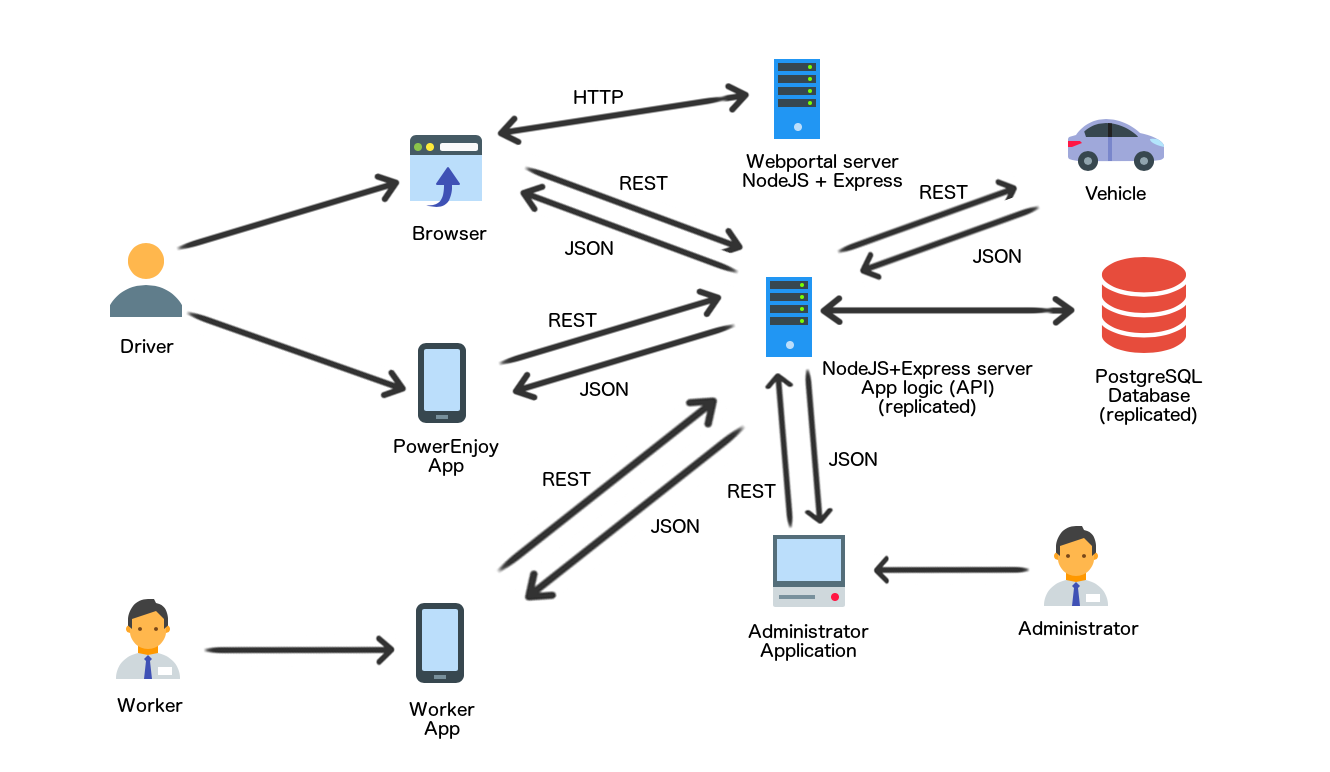
\includegraphics[width=13cm,keepaspectratio]{archi}

\section{High level components}
The high level structure of the System can be divided into 6 components. The main component is the \textbf{core}, that receives requests from \textbf{clients}, either \textbf{drivers}, \textbf{workers} and \textbf{administrators}; depending on the client type, the component provides different interfaces. 
The core also communicates with the \textbf{DBMS} component, responsible of data persistence. 
The core is also responsible of tracking vehicle states, by polling them every 30 seconds with a state request (HTTP GET).
The core implements all the business logic: 
\begin{itemize}
\item Process drivers requests and allocates the requested vehicle 
\item Manages vehicles, track their state
\item Manages users (drivers signup, login)
\item Manages reports and automatic tasks then it allocates them to workers
\end{itemize}
All the communications by clients (Driver, Worker, Admin) are realised in a synchronous client-server architecture, where the core is the server. The communications with the DBMS are also client-server (the core is the client) and are realised using PostgreSQL protocol. The communications with the vehicles uses HTTP but the core is the client, while vehicles are servers.

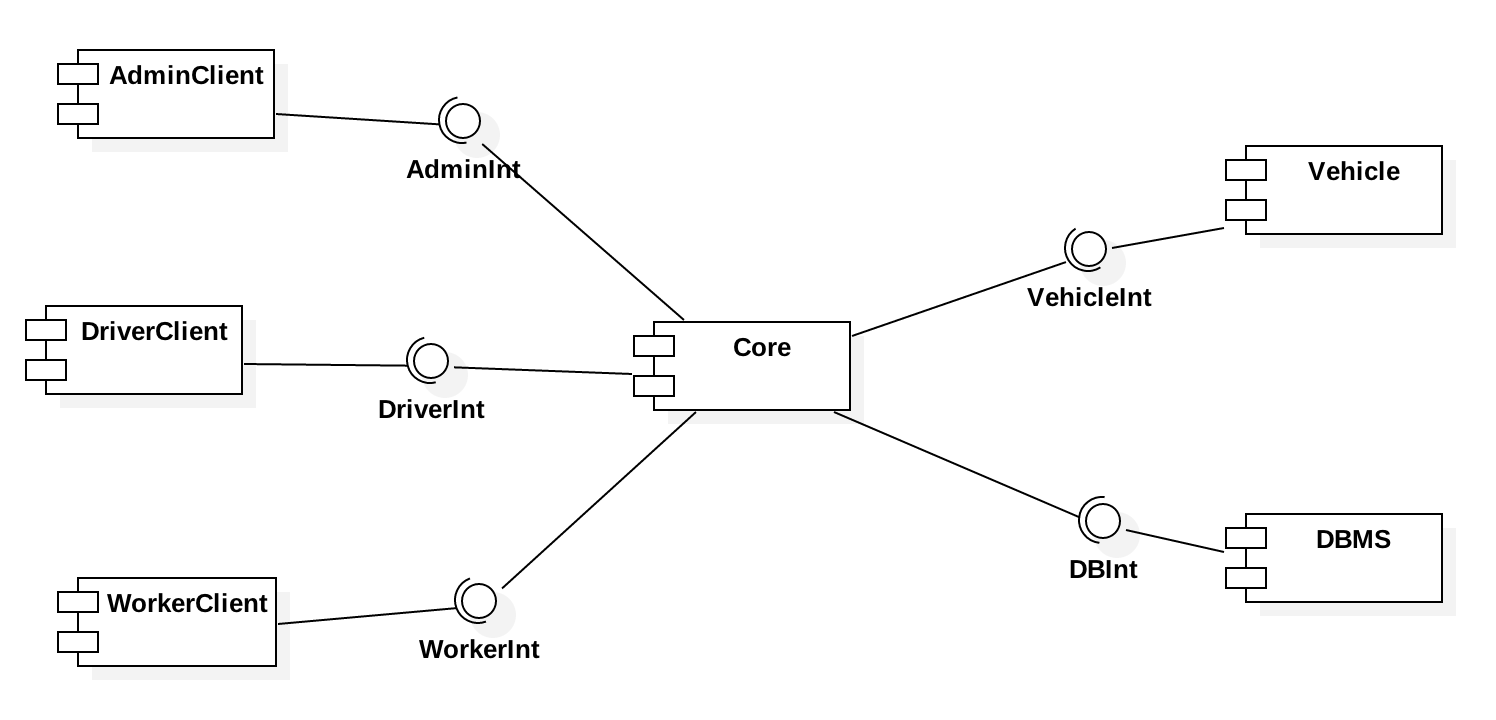
\includegraphics[width=13cm,keepaspectratio]{maincompo}

\subsection{Tracking vehicle state}
Tracking vehicle states requires a more detailed explanation. Our objective is to provide a simple interface for the core to communicate with vehicles (both tracking and controlling), so that the core can perform simple GET requests to endpoints (e.g. /vehicle/vehicle-id) to know their state (e.g. position, occupants) or POST request to perform actions on vehicles (e.g. open/close doors). Every vehicle is equipped with a wireless communication system, and is connected to the internet (so it has a public and static IP address). The core associate every vehicle ID with its IP address (and store this address in the DB), so every time a request to a specific vehicle is made, the core resolves the IP address of the requested vehicle. For security reasons, vehicles accept request only from the core IP (that is static). Every vehicle implements a simple on-board server, that answers to the core GET/POST requests, i.e. providing the vehicle's state or performing actions. 

\section {Core component}
Since the other components are quite simple and atomic, only the core component need some further analysis. The core has many functionalities that are divided in different components (for component diagram, see picture XXX):
\begin{itemize}
\item \textbf{Vehicle Manager} This component is responsible of tracking vehicle usage state (see state chart, picture XXX) but also vehicle internal state (e.g. position). This states are saved to the DB to provide persistency but also analytics. 
\item \textbf{Drive Controller} This component is responsible of processing Drivers requests (e.g. reservation, cancellation, termination). It communicates with the Vehicle Manager to update vehicle state. It also communicates with the Payment Manager to process Drivers payments. It is also responsible of computing the correct amount due at the end of a drive: requesting data from Vehicle Manager, it needs to compute the base amount to pay but also verify if discounts apply. A pseudo-code implementation of the amount computing is provided in chapter XXX.
\item \textbf{Payment Manager} It receives request to make a specific user pay a specific amount, process the payment and store it in the DB if the payment was successful. It is also responsible of verifying with the pre-authorization if the Driver can pay. 
\item \textbf{Task Manager} It is primarily responsible of managing task allocation to workers, but also of processing Drivers reports and generate automatic Tasks on vehicles. A pseudo-code implementation of the worker choosing algorithm is provided in chapter XXX.
\item \textbf{Authorization Manager} It manages most of the security of the system. It is responsible of Drivers and Workers signup and login. It is also responsible of verifying that requests to the core are performed by an authorized user (e.g. Driver can't request Workers API) 
\end{itemize}